\subsection{Entity-Relationship Schema}

    \begin{center}
        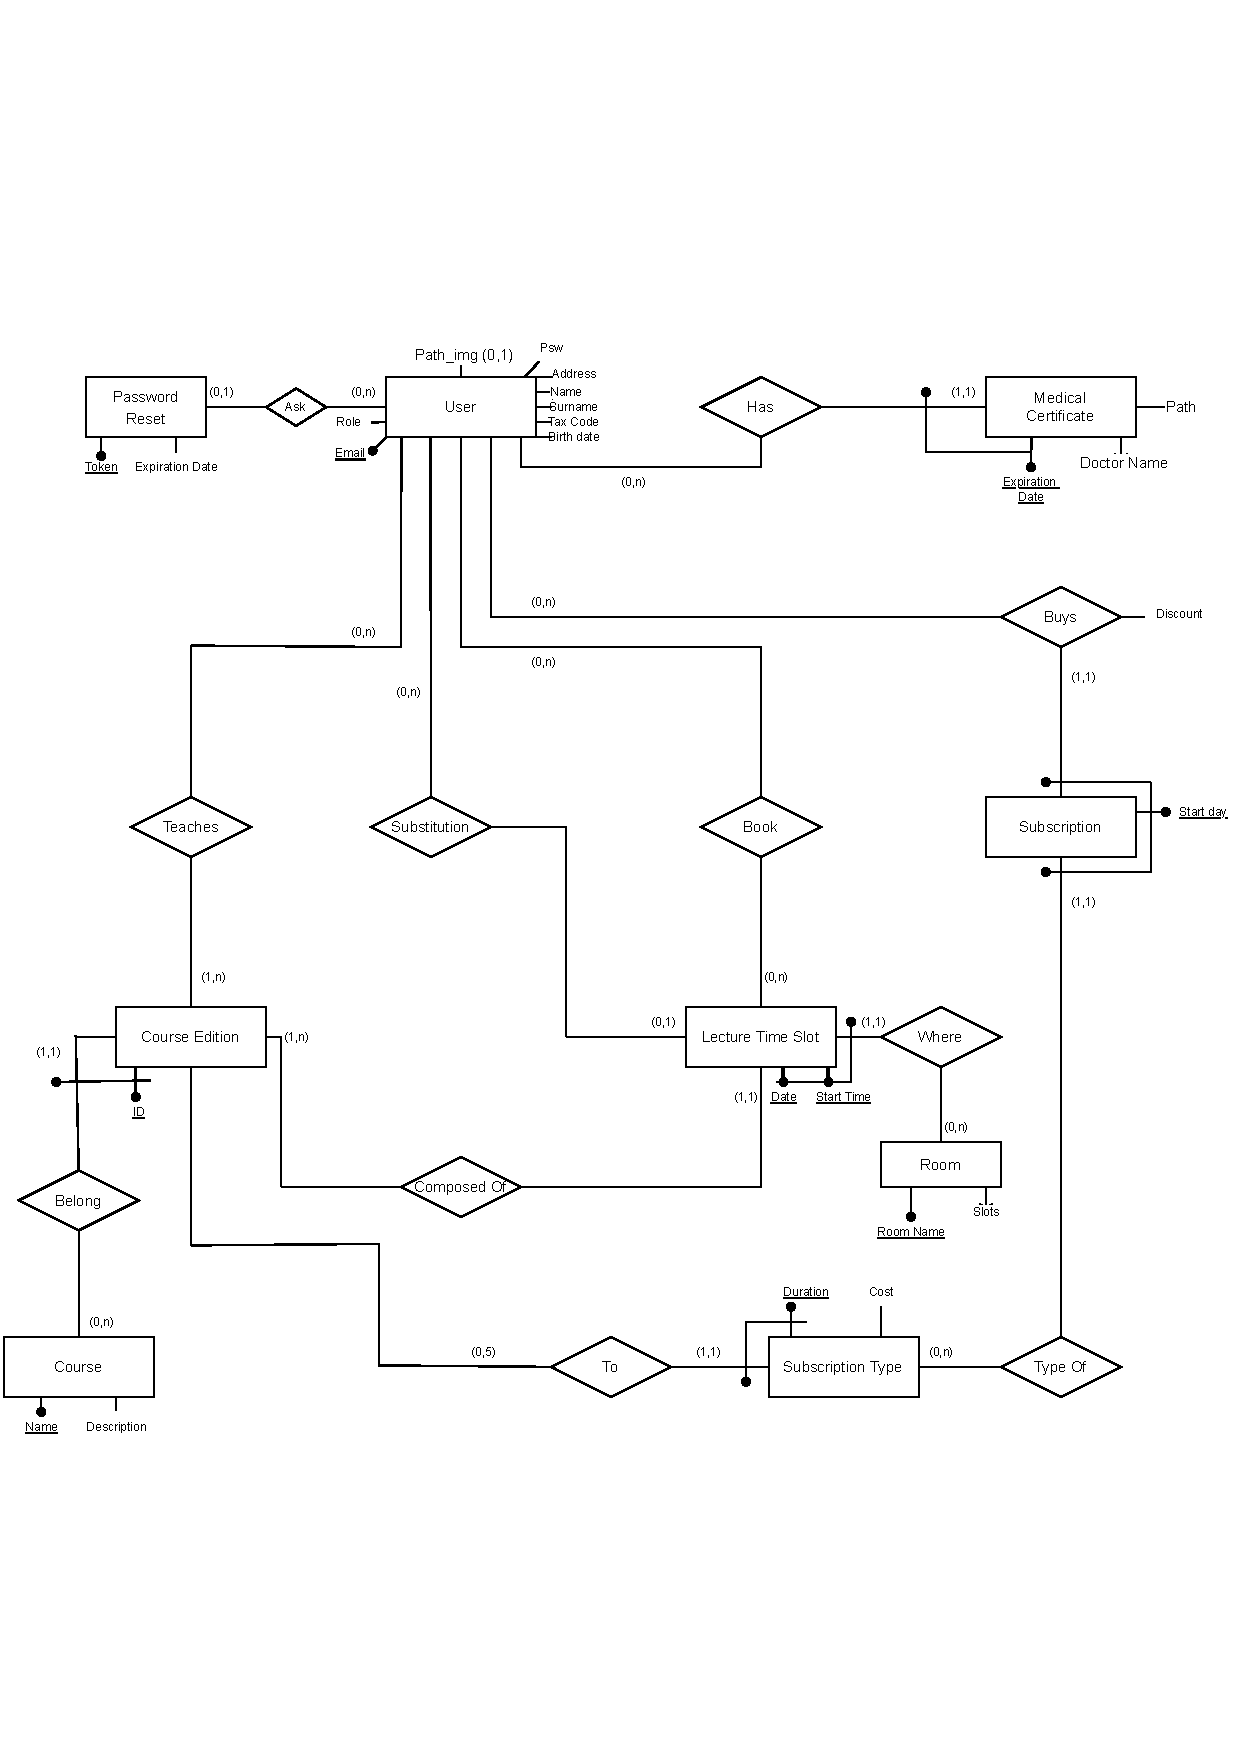
\includegraphics[width=0.9\textwidth]{resources/ER_restructured_v2.pdf}
        % this isn't finished yet
    \end{center}

    The entity-relationship contains 8 main entities:
    \begin{itemize}
        \item 
        \textbf{User}: each user of the application is identified by an \textit{Email} (type of VARCHAR). 
    	For each user we also save their \textit{Name}, \textit{Surname}, \textit{Address}, \textit{Telephone} and \textit{Path\textunderscore img} (for users's Profile image) as VARCHAR fields. We also save user's \textit{Birthday} (of type DATE). For each users we define
        one or more Roles (Indicated in the role attribute). The roles are:
        \begin{itemize}
	    \item Trainer: They held courses at the gym 
    	\item Trainee: Users which subscribes in order to partecipate to courses
        \item Secretary: Users that managed course subscriptions and in charge to sign presence
        
        \end{itemize}
    	\textcolor{red}{[ TODO restructuration: A: Each user can have one or more role among Trainer,  Trainee, and Secretary.\\
    	  B: Different entities Trainer,Trainee,Secretary. ]}
    	
    	\item 
    	\textbf{Course}: The gym has different courses and each of them is uniquely identified by 
    	\textit{Type Of Course} (type of VARCHAR). Each course also has and additional attribute \textit{Description} of type VARCHAR.
    	
    	\item 
    	\textbf{Course Edition}: Each course may have many course editions. Each course eddition is identified by the \textit{Year}(of type SMALLINT), and \textit{Course(Type Of Course)}.
    	
    	\item 
    	\textbf{Room}: Lessons of each course are held in a Room which is identified by its \textit{Name} (type of VARCHAR). Each room has also a boolean attribute, \textit{Slot Available}, for it's current availability.
    	
    	\item \textbf{Lecture Time Slot}: each Lecture Time Slot is identified by \textit{Room(name)}
    	
    	\item \textbf{Subscription Type}: each Subscription Type has \textit{Duration} and \textit{Cost}, both INTEGER fields. Every Subscription Type is identified by the \textit{Course(Type Of Course)} and its \textit{Duration}.
    	
    	\item \textbf{Subscription}: Every subscription has \textit{Month} and \textit{Year} attributes (both type of SMALLINT). Each trainee can have many Subscription to the gym and each trainee's subscription is identified by trainee's \textit{ID}, \textit{Month}, \textit{Year} and Subscription\textunderscore type's identification key \textit{(Duration, Course(Type Of Course))}.
    	
    	\item \textbf{Password Reset}: Additional entity to allow users to reset their password. It's identified by the \textit{Token} (type of VARCHAR) and three additional attributes: \textit{Expires} (type of TIMESTAMP), \textit{Used} and \textit{Revoked} both BOOLEAN fields.
        
        \item \textbf{Medical Certificate}: Entity used to store the medical certificate of a given user. It's identified by the \textit{User (ID)} and by the \textit{Expiring Date} (type of TIMESTAMP). It has two additional attributes: \textit{Doctor Name} (type of VARCHAR) and \textit{Path} (type of VARCHAR).
        	
    	% TODO THESE
    	\color{red}
    	\item[?]
    	\item \textbf{Medical\textunderscore certificate}
    	
    	\item \textbf{Lecture\textunderscore time\textunderscore slot} or
		\begin{itemize}
    	    \item \textbf{Session}
		    \item \textbf{Session\textunderscore canceled}
		    \item \textbf{Lecture}
		    \item \textbf{Reservation}
    	\end{itemize}
		\color{black}
	
    \end{itemize}